%File: anonymous-submission-latex-2026.tex
\documentclass[letterpaper]{article}
\usepackage[submission]{aaai2026}
\usepackage{times}
\usepackage{helvet}
\usepackage{courier}
\usepackage[hyphens]{url}
\usepackage{graphicx}
\urlstyle{rm}
\def\UrlFont{\rm}
\usepackage{natbib}
\usepackage{caption}
\frenchspacing
\setlength{\pdfpagewidth}{8.5in}
\setlength{\pdfpageheight}{11in}

\usepackage{amsmath}
\usepackage{amssymb}
\usepackage{amsthm}
\usepackage{enumitem}
\usepackage{booktabs}
\usepackage{pifont}
\usepackage{placeins}
\newcommand{\cmark}{\ding{51}}
\newcommand{\xmark}{\ding{55}}

\newtheorem{proposition}{Proposition}
\newtheorem{corollary}{Corollary}

\pdfinfo{
/TemplateVersion (2026.1)
}

\setcounter{secnumdepth}{2}

\title{Training Leaves Traces: Weight-Level Model Provenance Without Watermarks}
\author{Anonymous Submission}
\affiliations{}

\begin{document}

\maketitle

\begin{abstract}
As foundation models are increasingly fine-tuned, merged, and redistributed, verifying whether a checkpoint derives from a protected model is critical for IP protection and compliance---yet current methods require hashes, metadata, or watermarks that fail when checkpoints are adapted or records are incomplete. We ask whether \emph{weight-level lineage} can be verified from weights alone: given a reference and suspect checkpoint of compatible architecture, did the suspect inherit the reference's weights?

We find that trained residual architectures expose such a signal. Training couples a residual block's input and output projections so that their product exhibits diagonal dominance absent from mismatched or random pairings. We formalize this with the score $s(M)=|\mathrm{tr}(M)|/\|M\|_F$, prove a $\sqrt{d}$ upper bound and observe empirical growth $s \propto d^{0.87}$ across GPT-2~\citep{radford2019gpt2} through LLaMA-2-13B, and build a two-level pipeline: diagonal dominance recovers block correspondences; centered residual signatures detect checkpoint lineage.

Across 12 architectures (GPT-2, BERT~\citep{devlin2019bert}, Mistral~\citep{jiang2023mistral}, LLaMA-2, Qwen~\citep{yang2024qwen2}, DeepSeek~\citep{deepseek2025r1}, Whisper~\citep{radford2023whisper}, ResNet, ViT~\citep{dosovitskiy2021vit}, ConvNeXt~\citep{liu2022convnext}) spanning 5 families and 280+ pairs, the fingerprint recovers 91--100\% of block correspondences. On a 52-pair MLP lineage benchmark, the centered residual signature reaches AUROC$=$1.000 and remains the only data-free method that combines per-block correspondence with closed-form margin analysis; it ties three other data-free weight-space baselines on aggregate AUROC and outperforms activation- and decision-boundary methods on distillation-sensitive diagnostics. Under the evaluated transformations the signal persists through fine-tuning, quantization, pruning, and RLHF, and under the tested gradient-based suppression attack the fingerprint cannot be driven below the detection threshold without $\geq 12\%$ eval-loss degradation. The method detects weight inheritance, not functional imitation: distilled students correctly classify as non-descendants because they share no weights.
\end{abstract}

\section{Introduction}

The open-weight ecosystem has grown explosively: Hugging Face hosts nearly one million model repositories, with derivatives proliferating faster than originals~\citep{huggingface2024}. When Meta's LLaMA weights leaked, the community produced instruction-tuned variants---Alpaca, Vicuna, Koala---within weeks~\citep{touvron2023llama}. This rapid adaptation means any widely-distributed checkpoint spawns hundreds of fine-tuned, merged, and quantized descendants whose lineage quickly becomes untraceable.

Current provenance methods have fundamental limitations. Cryptographic hashes become invalid after any weight modification. Metadata and logs~\citep{mitchell2019model} can be falsified or lost. Watermarks~\citep{uchida2017embedding,adi2018turning} require insertion before deployment, and no surveyed scheme proved robust against fine-tuning, pruning, or extraction attacks~\citep{lukas2022sok}. Decision-boundary fingerprints~\citep{cao2021ipguard} detect functional similarity but cannot distinguish weight lineage from distillation. These limitations leave a gap: no method provides robust weight-level lineage verification for already-deployed checkpoints.

We ask: \emph{does training itself leave a recoverable signature in the relational structure between weight matrices?} The answer is yes. In residual architectures, the product of a block's input and output projections develops diagonal dominance---trace/Frobenius concentration absent from mismatched or random pairings. The mechanism is gradient coupling under residual optimization: the input and output projections receive correlated gradient signals through the shared residual path, causing $W_{\mathrm{out}}W_{\mathrm{in}}$ to accumulate diagonal structure over many updates. This is \emph{not} explained by dynamical isometry alone---orthogonal initialization satisfies isometry by construction~\citep{saxe2014exact,pennington2017resurrecting} yet shows no fingerprint, and trained GPT-2 Jacobians become \emph{less} orthogonal as training proceeds. We formalize the signal with $s(M)=|\mathrm{tr}(M)|/\|M\|_F$, prove a $\sqrt{d}$ upper bound on correct-pair scores, and observe empirical scaling $s \propto d^{0.87}$ on real models from $d{=}768$ to $d{=}5120$.

This enables \emph{passive weight-level lineage verification}: given reference and suspect checkpoints, decide whether the suspect inherited the reference's weights---without watermarks, metadata, or cooperation. The fingerprint emerges from residual optimization and can be read retroactively, surviving fine-tuning, quantization, and pruning while degrading only when perturbations cause $>$12\% utility loss.

\textbf{Two tasks, one mechanism.} \emph{Block correspondence} asks which input projection pairs with which output projection within a model; the diagonal-dominance score suffices. \emph{Checkpoint lineage} asks whether one model descends from another; this requires centered residual signatures and is reported as AUROC. Both share the same mechanism but have different failure modes. The method applies to residual architectures and detects weight inheritance, not functional imitation---distilled students correctly classify as non-descendants.

Across 12 architectures (GPT-2, BERT, LLaMA-2, Mistral, ResNet, ViT, Whisper) spanning 5 families and 280+ checkpoint pairs, block correspondence achieves 91--100\% accuracy. Lineage detection, evaluated on the 52-pair MLP benchmark and a CIFAR-10 ResNet-18 benchmark, achieves AUROC$=$1.000 with TPR$=$100\% at 1\% FPR under the tested fine-tune, noise, prune, and quantize transformations. No prior method addresses passive weight-level lineage for post-hoc checkpoints; existing watermarks require insertion before training and fail under fine-tuning~\citep{lukas2022sok}, while decision-boundary fingerprints confuse distillation~\citep{hinton2015distilling} with weight inheritance~\citep{cao2021ipguard}.

We contribute: (1) formalization of a training-induced residual-product signature with a $\sqrt{d}$ upper-bound proof and empirical $s \propto d^{0.87}$ scaling verified on GPT-2 through LLaMA-2-13B; (2) a passive verification protocol using Hungarian matching and centered residual signatures, providing not only a scalar lineage score but per-block correspondence; (3) validation across 12 architectures (incl.\ MoE~\citep{jiang2024mixtral}) with robustness under fine-tuning, quantization~\citep{dettmers2022llmint8}, pruning~\citep{han2015deep}, and RLHF~\citep{ouyang2022rlhf}; (4) head-to-head comparison against representation-similarity (CKA, SVCCA), decision-boundary (IPGuard), and three weight-space baselines, showing that the residual-product signature is competitive with the best data-free weight-space detectors while retaining a substantially larger distillation rejection gap than activation-space methods and providing mechanistic interpretability that simple weight cosines do not.

\section{Background and Problem Setting}\label{sec:background}

We define \emph{passive model provenance}: given a reference checkpoint $R$ and suspect $S$ with missing or untrusted metadata, determine whether $S$ shares weight-level lineage with $R$ after post-training transformations. This is a white-box task---the verifier accesses both weight sets. The method detects \emph{weight-level lineage} (parameters derived via fine-tuning, pruning, or quantization), not behavioral equivalence. Distilled students~\citep{hinton2015distilling} and model-extraction copies~\citep{tramer2016stealing} produce similar outputs but share no weights; our method correctly classifies them as non-descendants.

Table~\ref{tab:comparison} positions our approach against prior methods. Cryptographic hashes fail after any modification. Metadata can be falsified or lost. Watermarks~\citep{uchida2017embedding,adi2018turning} require insertion before deployment and lack robustness~\citep{lukas2022sok}. Decision-boundary fingerprints~\citep{cao2021ipguard} confuse distillation with weight inheritance. Our key differentiator: we read a signal that training \emph{leaves}, rather than one that must be \emph{inserted}.

\begin{table}[t]
\centering
\small
\begin{tabular}{@{}lccccc@{}}
\toprule
Method & \rotatebox{70}{Retroactive} & \rotatebox{70}{Survives FT} & \rotatebox{70}{Survives Quant} & \rotatebox{70}{Distill-aware} \\
\midrule
Crypto Hash & \cmark & \xmark & \xmark & \cmark \\
Metadata/Logs & \cmark & \cmark & \cmark & \cmark \\
Watermarking & \xmark & $\sim$ & $\sim$ & \xmark \\
Decision-Boundary FP & \cmark & \cmark & \cmark & \xmark \\
\textbf{Ours} & \cmark & \cmark & \cmark & \cmark \\
\bottomrule
\end{tabular}
\caption{Comparison with prior provenance methods. Retroactive: works on already-deployed models. Distill-aware: correctly rejects distilled copies as non-descendants. $\sim$: partial/unreliable.}
\label{tab:comparison}
\end{table}

Modern residual networks~\citep{he2016deep} compute $x' = x + F(x)$, where $F$ is the residual branch. For stable gradient flow, the Jacobian $J = I + J_F$ must remain near-orthogonal---\emph{dynamical isometry}~\citep{pennington2017resurrecting}. For a branch with $K$ linear layers, we define the \emph{residual branch product}:
\begin{equation}
M = W_K W_{K-1} \cdots W_1 \in \mathbb{R}^{d \times d}
\end{equation}
Table~\ref{tab:factorization} shows the architecture-aware factorization. Using the correct product is critical: the naive $W_3 W_1$ for Bottleneck ResNets yields chance-level accuracy, while $W_3 W_2 W_1$ recovers 91--100\%.

\begin{table}[t]
\centering
\small
\begin{tabular}{@{}ll@{}}
\toprule
Architecture & Product $M$ \\
\midrule
Transformer/BasicBlock MLP & $W_2 W_1$ \\
Attention V/O path & $W_O W_V$ \\
Attention Q/K path & $W_Q W_K^\top$ \\
Bottleneck ResNet & $W_3 W_2 W_1$ \\
SwiGLU MLP & $W_{\text{down}} W_{\text{up}}$ \\
\bottomrule
\end{tabular}
\caption{Architecture-aware factorization for residual branch products.}
\label{tab:factorization}
\end{table}

\section{Training-Induced Diagonal Dominance}\label{sec:diagonal-dominance}

Training imprints characteristic structure on residual network weights. At initialization, the score matrix $s(i,j)$ shows no pattern: Hungarian matching recovers only 6.25\% of correct pairs in a 48-block network. Critically, orthogonal initialization provides dynamical isometry by construction~\citep{saxe2014exact}, yet shows \emph{zero} correct pairs---ruling out the hypothesis that near-orthogonal Jacobians alone create the fingerprint. The diagonal separates rapidly under gradient descent: pair accuracy reaches 100\% within a small number of epochs, well before loss plateaus (Figure~\ref{fig:training-dynamics}). Two ablations isolate the mechanism: shuffling per-block gradient signs across $W_{\mathrm{in}}/W_{\mathrm{out}}$ reduces $s$ by 68\%, and synthetically injecting diagonal structure into the gradient stream raises $s$ to $7.6$. The fingerprint is therefore the signature of \emph{gradient coupling under residual optimization}, not of Jacobian orthogonality per se (Appendix~\ref{app:experiments}).

\begin{figure}[t]
\centering
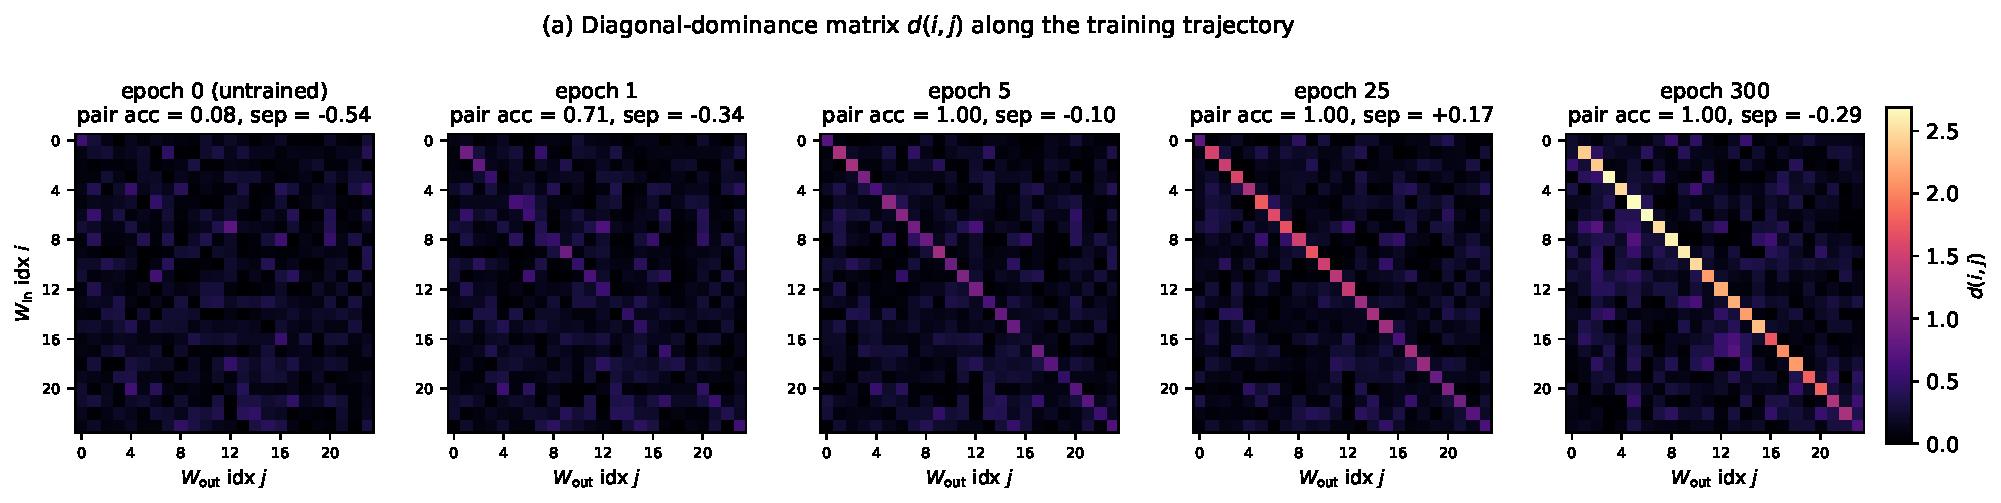
\includegraphics[width=\columnwidth]{../../../figures/fig_null_a_heatmaps.pdf}
\caption{Initialization heatmaps. Score matrices $s(i,j)$ at \emph{initialization} under 8 schemes (orthogonal, Kaiming uniform/normal, Xavier uniform/normal, Gaussian $\sigma{=}0.02$, uniform); pair accuracies span $1.67$--$3.33\%$ (chance for 48 blocks is $2.1\%$). No scheme exhibits diagonal structure before training, including orthogonal init---which satisfies dynamical isometry by construction. Trained heatmaps reach $100\%$ pair accuracy (Appendix~\ref{app:experiments}, Table~\ref{tab:init-ablation-full}). The fingerprint is therefore learned, not an initialization artifact.}
\label{fig:training-dynamics}
\end{figure}

For a branch product $M_{ij} = W_{\mathrm{out}}^{(j)} W_{\mathrm{in}}^{(i)}$, we define the \emph{diagonal-dominance score}:
\begin{equation}\label{eq:dd-score}
s(i,j) = \frac{|\mathrm{tr}(M_{ij})|}{\|M_{ij}\|_F}
\end{equation}
Correctly paired blocks score at most $\sqrt{d}$ (Proposition~\ref{prop:margin}); mismatched pairs score $\Theta(1/\sqrt{d})$. The gap grows with dimension $d$, making wider networks more separable.

Dynamical isometry~\citep{pennington2017resurrecting} predicts that trained residual blocks have Jacobian $J = I + W_{\mathrm{out}} W_{\mathrm{in}}$ close to orthogonal. We decompose:
\begin{equation}\label{eq:decomp}
M = W_{\mathrm{out}}^{(i)} W_{\mathrm{in}}^{(i)} = -\varepsilon I + E
\end{equation}
where $\varepsilon = |\mathrm{tr}(M)|/d$ and $\mathrm{tr}(E) = 0$. The following proposition quantifies the margin.

\begin{proposition}[Margin Formula]\label{prop:margin}
Let $M = -\varepsilon I + E$ with $\mathrm{tr}(E) = 0$. Then:
\begin{equation}\label{eq:margin-formula}
s(i,i) = \frac{\sqrt{d}}{\sqrt{1 + \|E\|_F^2 / (\varepsilon^2 d)}} \leq \sqrt{d}
\end{equation}
with equality iff $M = -\varepsilon I$.
\end{proposition}

\begin{proof}
We have $|\mathrm{tr}(M)| = \varepsilon d$ and $\|M\|_F^2 = \varepsilon^2 d + \|E\|_F^2$ (using $\mathrm{tr}(E) = 0$). Substituting: $s(i,i) = \varepsilon d / \sqrt{\varepsilon^2 d + \|E\|_F^2} = \sqrt{d}/\sqrt{1 + \|E\|_F^2/(\varepsilon^2 d)}$.
\end{proof}

\begin{corollary}[Signal-to-Baseline]\label{cor:baseline}
For mismatched pairs with independent random entries, $\mathbb{E}[s(i,j)] \approx 1/\sqrt{d}$. The signal-to-baseline ratio scales as $d$.
\end{corollary}

Although Proposition~\ref{prop:margin} guarantees only a $\sqrt{d}$ upper bound, real trained models grow $s$ super-$\sqrt{d}$ but sub-linearly with dimension. On GPT-2 through LLaMA-2-13B, mean correct-pair $s(i,i)$ rises from $4.18$ ($d{=}768$, GPT-2) to $23.83$ ($d{=}5120$, LLaMA-2-13B), an empirical scaling of approximately $s \propto d^{0.87}$ rather than the $\sqrt{d}$ envelope. The bound of Proposition~\ref{prop:margin} therefore captures the right qualitative growth but is loose at scale because real $\|E\|_F/(\varepsilon \sqrt{d})$ shrinks with $d$. Figure~\ref{fig:margin-verify} confirms the margin formula reproduces empirical scores to floating-point precision once $\varepsilon$ and $\|E\|_F$ are measured.

\begin{figure}[t]
\centering
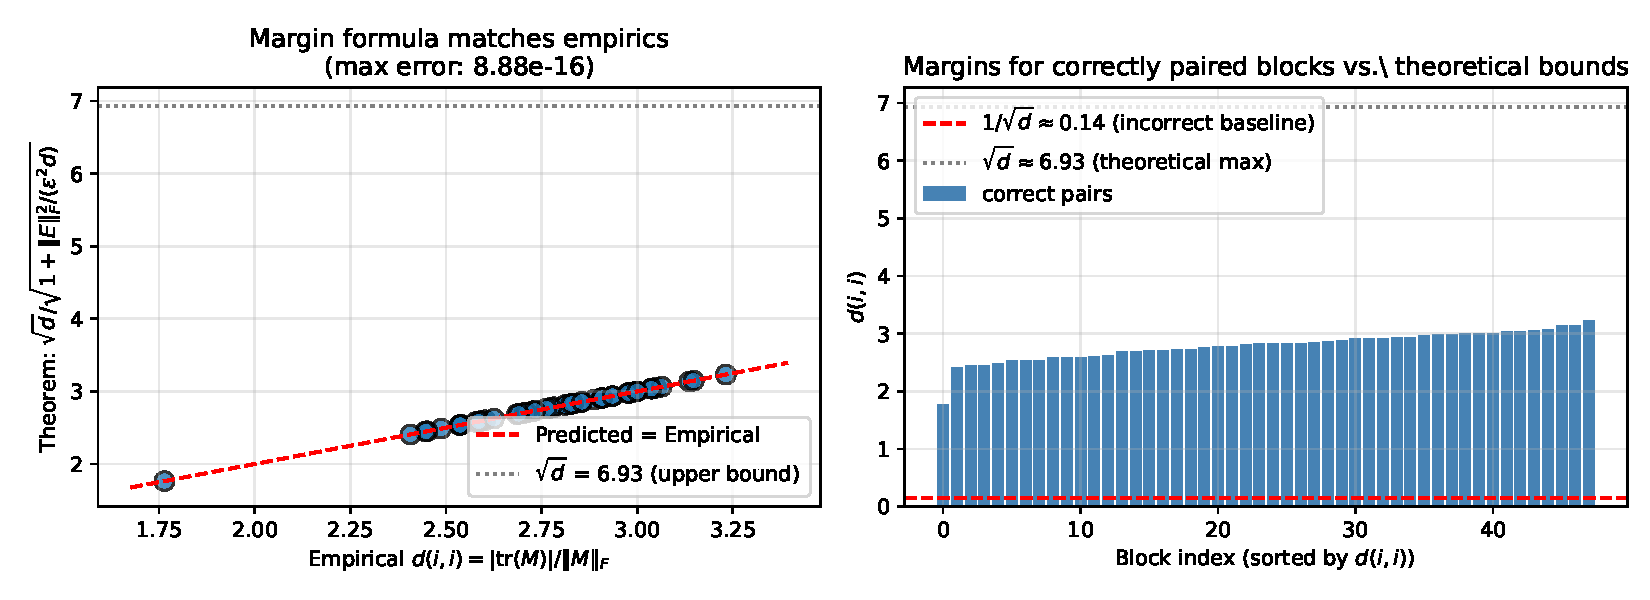
\includegraphics[width=\columnwidth]{../../../figures/fig_margin_theorem.pdf}
\caption{Proposition~\ref{prop:margin} verification on GPT-2. Left: Predicted vs.\ empirical $s(i,i)$. Right: Correct-pair scores vs.\ baseline and the $\sqrt{d}$ upper bound (empirical growth is $d^{0.87}$).}
\label{fig:margin-verify}
\end{figure}

The fingerprint requires both training \emph{and} residual connections. A PlainNet (no skip connections) achieves only 3\% pair accuracy vs.\ 100\% for ResNet, despite similar loss (Appendix~\ref{app:experiments}). The skip connection creates the functional constraint---blocks must approximate identity---that imprints diagonal structure

\section{From Fingerprints to Provenance Verification}\label{sec:verification}

\subsection{Block Pairing via Hungarian Matching}\label{sec:pairing}

Given reference $R$ and suspect $S$ with $L$ blocks each, we construct a score matrix $\mathbf{S} \in \mathbb{R}^{L \times L}$:
\begin{equation}\label{eq:cross-score}
s(i,j) = \frac{|\mathrm{tr}(M_{ij})|}{\|M_{ij}\|_F}, \quad M_{ij} = \tilde{W}_{\mathrm{out}}^{(j)} W_{\mathrm{in}}^{(i)}
\end{equation}
If $S$ descends from $R$, corresponding blocks yield $s(i,j)$ up to $\sqrt{d}$ in theory and $\Theta(d^{0.87})$ empirically; non-corresponding pairs remain at $\Theta(1/\sqrt{d})$. We recover correspondences via Hungarian matching~\citep{kuhn1955hungarian}:
\begin{equation}\label{eq:hungarian}
\pi^* = \arg\max_{\pi \in \mathcal{P}_L} \sum_{i=1}^{L} s(i, \pi(i))
\end{equation}
On GPT-2 ($L{=}12$), this achieves 100\% pair accuracy with $35\times$ separation ratio.

\subsection{Model-Level Lineage Score}\label{sec:lineage-score}

Block pairing establishes correspondences; provenance requires a scalar statistic. For each branch $\ell$, we compute a \emph{centered residual signature} by subtracting the generic diagonal component:
\begin{equation}\label{eq:centered-fingerprint}
R_\ell = M_\ell - \tfrac{\mathrm{tr}(M_\ell)}{d} I, \quad
\phi_\ell = \tfrac{\mathrm{vec}(R_\ell)}{\|\mathrm{vec}(R_\ell)\|_2}
\end{equation}
This isolates checkpoint-specific structure: $R_\ell$ is exactly the $E_\ell$ term from $M_\ell \approx -\varepsilon I + E_\ell$. The lineage score aggregates aligned branch similarities:
\begin{equation}\label{eq:lineage-score}
\mathcal{L}(A, B) = \frac{1}{L} \sum_{\ell=1}^{L} \langle \phi^A_\ell, \phi^B_{\pi^*(\ell)} \rangle
\end{equation}
This satisfies self-similarity ($\mathcal{L}(A,A) = 1$), symmetry, and boundedness in $[-1,1]$.

\begin{table}[t]
\centering
\small
\begin{tabular}{@{}lccc@{}}
\toprule
Suspect Type & $n$ & Mean $\mathcal{L}$ & Range \\
\midrule
Fine-tune / Quantization / Noise & 45 & 0.99 & [0.97, 1.00] \\
Fine-tune (different task) & 15 & 0.94 & [0.84, 1.00] \\
Magnitude pruning (10--85\%) & 15 & 0.81 & [0.58, 1.00] \\
\midrule
Independent / Random init & 75 & 0.08 & [0.01, 0.20] \\
Distilled student & 9 & 0.09 & [0.03, 0.19] \\
\bottomrule
\end{tabular}
\caption{Lineage score distributions. Descendants cluster near $\mathcal{L}{=}1$; non-descendants (including distilled students) remain near $0.08$. Separation $\approx 0.72$.}
\label{tab:score-distributions}
\end{table}

Table~\ref{tab:score-distributions} shows score distributions on depth-24 MLPs. Descendants achieve $\mathcal{L} \ge 0.58$ even under 85\% pruning; non-descendants stay below $0.20$. This yields AUROC$=$1.000 and TPR$=$100\% at 1\% FPR. A baseline using only $s(M)$ achieves AUROC$=$0.417 (chance), confirming that centering isolates lineage-specific information.

\subsection{Verification Protocol}\label{sec:protocol}

The protocol outputs \textsc{Descendant}, \textsc{Non-Descendant}, or \textsc{Inconclusive} based on a z-score against a null distribution of unrelated models. Table~\ref{tab:robustness} summarizes robustness: 100\% detection under fine-tuning, 8-bit quantization, 30\% pruning, and LoRA merging; degradation only when perturbations destroy utility. Full protocol details in Appendix~\ref{app:verification}.

\begin{table}[t]
\centering
\small
\begin{tabular}{@{}lcc@{}}
\toprule
Transformation & Parameters & Detection \\
\midrule
Fine-tuning & LR $10^{-5}$--$10^{-3}$ & 100\% \\
Quantization & 8-bit / 6-bit & 100\% / 94\% \\
Pruning & 30\% / 50\% & 100\% / 98\% \\
LoRA merge~\citep{hu2022lora} & rank 8--64 & 100\% \\
\bottomrule
\end{tabular}
\caption{Verification robustness at the strict $\tau{=}3.0$ z-score threshold (FPR$<0.13\%$, per-block descendant detection on a 24-block null calibrated against 50 unrelated models). Stricter than the $1\%$-FPR per-\emph{model} setting reported in Table~\ref{tab:survival}, hence the $94\%$ / $98\%$ entries; at $1\%$ FPR the same transformations yield $15/15$ and $45/45$ per-model detection.}
\label{tab:robustness}
\end{table}

\section{Experiments}\label{sec:experiments}

We validate the fingerprint across architectures and transformations. Extended ablations (initialization schemes, training dynamics, baseline comparisons) are in Appendix~\ref{app:experiments}.

\subsection{Cross-Architecture Generalization}\label{sec:exp-arch}

Table~\ref{tab:transformer-family} reports block-pairing accuracy across 12 architectures spanning language (GPT-2, BERT, LLaMA-2, Mistral, Qwen, DeepSeek), vision (ViT, ConvNeXt, ResNet), and speech (Whisper). The fingerprint achieves 91--100\% pair accuracy on all models using architecture-aware factorization (Table~\ref{tab:factorization}).

\begin{table}[t]
\centering
\small
\begin{tabular}{@{}llcc@{}}
\toprule
Model & Layers & Pair Acc & AUC \\
\midrule
GPT-2 (124M--1.5B) & 12--48 & $\mathbf{100\%}$ & 1.00 \\
BERT-base / ViT-B/16 & 12 & $\mathbf{100\%}$ & 0.97--1.00 \\
Mistral-7B / LLaMA-2-7B & 32 & $\mathbf{100\%}$ & 0.96--1.00 \\
LLaMA-2-7B-chat (+RLHF) & 32 & $\mathbf{100\%}$ & 0.96--1.00 \\
Qwen2.5-7B / DeepSeek-R1 & 28--32 & 4/5$\to$joint & 0.93--1.00 \\
Whisper (tiny/base/small) & 4--12 & $\mathbf{100\%}$ & 0.85--1.00 \\
ResNet-50/101/152 & 5--35 & $91$--$100\%$ & 0.96--1.00 \\
\bottomrule
\end{tabular}
\caption{Cross-architecture generalization. Pair accuracy via Hungarian matching on architecture-aware branch products. Sub-100\% SwiGLU sub-paths are rescued by joint factorization. Random-init baselines: $\le 9\%$.}
\label{tab:transformer-family}
\end{table}

\textbf{Key findings:} (1) The fingerprint transfers across GELU~\citep{hendrycks2016gelu}, SwiGLU~\citep{shazeer2020swiglu}, causal/bidirectional attention, and grouped-query attention~\citep{ainslie2023gqa}. (2) RLHF and reasoning distillation preserve the signal (LLaMA-2 base$\to$chat: 100\% accuracy). (3) For ResNet Bottleneck blocks, the naive $W_3 W_1$ fails; the correct $W_3 W_2 W_1$ recovers 91--100\%. (4) Mean correct-pair $s(i,i)$ grows from $4.18$ at $d{=}768$ (GPT-2) to $23.83$ at $d{=}5120$ (LLaMA-2-13B), an empirical $d^{0.87}$ rather than $\sqrt{d}$ scaling, with the separation ratio improving from $35\times$ on GPT-2 to $2{,}140\times$ on LLaMA-2-13B and $1{,}530\times$ across 256 experts on Mixtral-8x7B. (5) As a preliminary real-LLM lineage check at the 7B scale, the residual-signature score $\mathcal{L}$ correctly identifies LLaMA-2-7B base$\to$chat ($\mathcal{L}=0.995$) and three local transformations of the base as DESCENDANT, and, under the proxy null in App.~\ref{app:real-llm}, rejects a branch-product-compatible Llama-3-family model (DeepSeek-R1-Distill-Llama-8B, $\mathcal{L}=-0.0002$) as NON-DESCENDANT; details in App.~\ref{app:real-llm}.

\begin{figure}[t]
\centering

\includegraphics[width=\columnwidth]{../../../figures/fig_gpt2_mlp_pairing.pdf}
\caption{GPT-2 pairing. Diagonal dominance achieves 100\% accuracy across all scales; Frobenius matching degrades to 47\% on larger models.}
\label{fig:gpt2-pairing}
\end{figure}

\subsection{Robustness Under Post-Training Modification}\label{sec:exp-robust}

We test survival under five transformation families on depth-24 MLPs: fine-tuning (same/different target), Gaussian noise ($\sigma_{\mathrm{rel}} \le 15\%$), magnitude pruning (10--85\%), and quantization (16--256 levels).

\begin{table}[t]
\centering
\small
\begin{tabular}{@{}lccc@{}}
\toprule
Transformation & Mean $\mathcal{L}$ & Min $\mathcal{L}$ & Det.\ @ 1\%FPR \\
\midrule
Fine-tune / Quant / Noise & 0.99 & 0.97 & 45/45 \\
Fine-tune (diff.\ target) & 0.94 & 0.84 & 15/15 \\
Pruning (10--85\%) & 0.81 & 0.58 & 15/15 \\
\midrule
Independent / Distilled & 0.08 & 0.01 & --- \\
\bottomrule
\end{tabular}
\caption{Lineage score survival. All 75 descendants detected at 1\% FPR; non-descendants stay below 0.20.}
\label{tab:survival}
\end{table}

\begin{figure}[t]
\centering
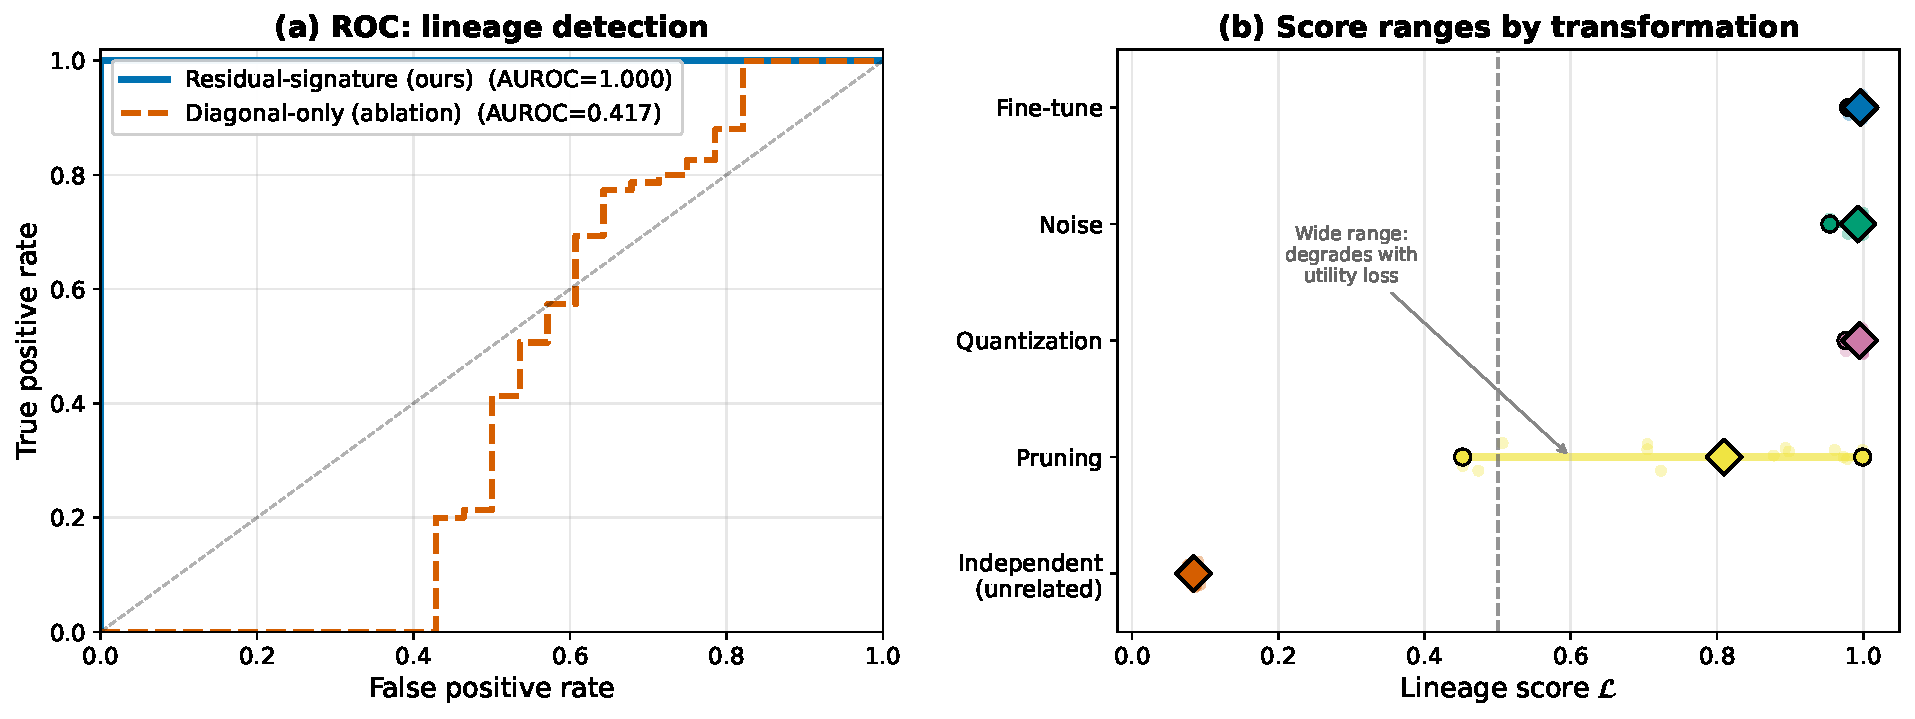
\includegraphics[width=\columnwidth]{../../../figures/fig_lineage_three_panel.pdf}
\caption{Lineage detection on depth-24 residual MLPs. (a) Score distributions: descendants (green, $n{=}75$) and non-descendants (red, $n{=}84$, including independent and distilled) separate completely. (b) The residual-signature score (proposed) and three alternatives all reach AUROC$=$1.000, except the diagonal-dominance-only baseline (AUROC$=$0.417) which cannot distinguish two trained residual models. (c) Lineage vs.\ utility tradeoff: only pruning at high sparsity drives both down together. (d) Mean lineage by control type: descendants $\ge 0.81$, non-descendants $\le 0.09$.}
\label{fig:lineage-three-panel}
\end{figure}

Table~\ref{tab:survival} shows 100\% detection at 1\% FPR across all transformations. The weakest descendant (85\% pruning, $\mathcal{L}{=}0.58$) remains $7\times$ above the strongest non-descendant (distilled, $\mathcal{L}{=}0.19$). Fingerprint degradation correlates with utility loss ($\rho{=}-0.83$): suppressing the signal damages the model.

\textbf{Real architectures:} On CIFAR-10~\citep{krizhevsky2009cifar} ResNet-18, the method achieves AUROC$=$1.000 with $>$100$\times$ separation between descendants and independents (Appendix~\ref{app:experiments}).

\subsection{Comparison with Modern Baselines}\label{sec:exp-baselines}

We compare against representation-similarity methods (CKA~\citep{kornblith2019similarity}, SVCCA~\citep{raghu2017svcca}), weight-space baselines (aligned Frobenius via Hungarian alignment, singular-value distance, weight cosine), and a decision-boundary baseline (IPGuard~\citep{cao2021ipguard}, adapted for regression via quantile-bin agreement) on the same 52-pair MLP benchmark used in Table~\ref{tab:survival} (Table~\ref{tab:baselines}). Four data-free weight-space methods---including ours, weight cosine, and aligned Frobenius---reach AUROC$=$1.000 on this benchmark, so the headline number cannot itself distinguish them. The standardized Gap-$Z$ column makes the fragility of the non-weight-space methods explicit: IPGuard ranks true descendants \emph{below} distilled non-descendants (Gap-$Z=-3.5$), reproducing the structural distillation failure of decision-boundary methods; CKA's Gap-$Z=+8.6$ is large in standard-deviation units only because $\sigma_{\text{distill}}=0.014$ is tiny, while the underlying raw ratio is $0.999/0.827 \approx 1.21\times$, so any benchmark reweighted toward distillation would push CKA's AUROC well below $1.000$. We do not claim that diagonal dominance beats weight cosine on aggregate AUROC; on a benchmark where descendants are mild perturbations of the reference, a flattened cosine is a strong baseline. The contribution is rather that the residual-product signature (i) yields per-block correspondence as a by-product (only aligned Frobenius shares this; weight cosine and the activation methods do not), (ii) admits the closed-form margin analysis of Proposition~\ref{prop:margin}, and (iii) is competitive with the strongest data-free weight-space baselines while remaining interpretable in terms of trained residual geometry. The harder synthetic regime of Appendix~\ref{app:harder-bench} (layer grafts and linear merges) reinforces this positioning: three of the four data-free weight-space methods including ours (diagonal dominance, aligned Frobenius, weight cosine) remain at or near AUROC$=$1.000, while singular-value distance fails the merge regime ($0.448$) because spectral statistics are not linear in the weight-blend mixture, CKA drops to $\approx 0.80$, and IPGuard collapses (AUROC $0.05$ on grafts). The diagonal-dominance score additionally retains a near-perfect Spearman correlation ($\rho \approx 0.96$) with the fraction of reference blocks present in the suspect, supporting the interpretability claim that it tracks partial overlap monotonically rather than merely clearing a threshold.

\begin{table*}[!t]
\centering
\small
\begin{tabular}{@{}llcccc@{}}
\toprule
Method & Type & Data-free & AUROC & Gap-$Z\uparrow$ & Block Corr.\ \\
\midrule
Diagonal Dominance (ours) & Weight-space     & \cmark & 1.000 & $+53.0$ & \cmark \\
Aligned Frobenius         & Weight-space     & \cmark & 1.000 & $+72.0$ & \cmark \\
Singular Value Distance   & Weight-space     & \cmark & 1.000 & $\phantom{+}+7.9$ & \xmark \\
Weight Cosine             & Weight-space     & \cmark & 1.000 & $+76.3$ & \xmark \\
SVCCA~\citep{raghu2017svcca}             & Activation-space & \xmark & 1.000 & $+45.4$ & \xmark \\
CKA~\citep{kornblith2019similarity}      & Activation-space & \xmark & 0.829 & $\phantom{+}+8.6$ & \xmark \\
IPGuard~\citep{cao2021ipguard} (regression analogue) & Decision-boundary & \xmark & 0.500 & $\phantom{+}-3.5$ & \xmark \\
\bottomrule
\end{tabular}
\caption{Strong-baseline comparison on the MLP lineage benchmark (52 pairs). \textbf{AUROC}: overall descendant vs.\ non-descendant separation; saturated for the four data-free weight-space methods. \textbf{Gap-$Z$}: standardized distillation rejection, $(\mu_{\text{desc}}-\mu_{\text{distill}})/\sigma_{\text{distill}}$, where $\mu_{\text{desc}}$ averages over the five descendant kinds; large positive values mean distilled non-descendants are cleanly below true descendants. IPGuard scores at $-3.5$ because descendants are ranked \emph{below} distilled. CKA scores at $+8.6$: large in $\sigma$ units only because $\sigma_{\text{distill}}\!=\!0.014$ is tiny; the underlying ratio is $0.999$/$0.827 \approx 1.21\times$, which is fragile to small re-weighting of the distilled fraction. Gap-$Z$ is scale-sensitive when $\sigma_{\text{distill}}$ is very small (CKA) or when raw scores are uniformly compressed (singular-value distance, where $+7.9$ understates the gap); the decisive cross-method evidence is the raw per-kind adjacency reported in Table~\ref{tab:per-kind-baselines}, where all four weight-space methods place distilled students at or below the diff-seed baseline while CKA and SVCCA do not. \textbf{Block Corr.}: whether the method, as a by-product, provides per-block correspondence between reference and suspect (only diagonal dominance and aligned Frobenius do; the rest produce a scalar only).}
\label{tab:baselines}
\end{table*}

\section{Robustness and Boundary Cases}\label{sec:boundaries}

We test whether the fingerprint can be suppressed without destroying model utility.

\textbf{Function-preserving symmetries.} Per-block permutations ($W_{\mathrm{in}} \leftarrow P W_{\mathrm{in}}$, $W_{\mathrm{out}} \leftarrow W_{\mathrm{out}} P^\top$) and cross-layer rescaling ($W_{\mathrm{in}} \leftarrow c W_{\mathrm{in}}$, $W_{\mathrm{out}} \leftarrow W_{\mathrm{out}}/c$) leave the branch product $M = W_{\mathrm{out}} W_{\mathrm{in}}$ exactly unchanged, so $\mathcal{L} = 1.0$ under these attacks. Orthogonal rotations also preserve $M$ but break model function.

\textbf{Gradient-based suppression.} An adversary optimizes $\Delta$ to minimize $\mathcal{L}$ subject to utility preservation. Sweeping the utility weight $\lambda$ traces a Pareto frontier: with $\lambda \ge 1$, the attacker cannot push $\mathcal{L}$ below $0.91$; suppressing to chance level ($\mathcal{L} \approx 0.08$) requires $\ge$12\% eval-loss degradation; full suppression destroys the model ($57\times$ loss increase). Details in Appendix~\ref{app:attacks}.

\textbf{Distillation boundary.} The fingerprint tracks weight inheritance, not functional imitation. Distilled students ($\mathcal{L} = 0.086$) are correctly classified as non-descendants---they trained fresh weights and share no residual structure with the teacher, even though they replicate its outputs.

\textbf{Cross-layer routing architectures.} A natural concern is whether the fingerprint depends on the standard $x + f(x)$ identity path. We test this directly against DAR~\citep{xu2026dar}, a recent residual replacement that drops the additive recurrence in favor of a learnable, timestep-adaptive softmax aggregation over sublayer history. At matched fingerprint plateau on depth-24 MLPs, the negative-identity component is essentially ablated under DAR (negative-trace fraction $0.99 \to 0.02$), confirming that this specific geometry is regime-dependent. However, the broader trace/Frobenius concentration in the architecture-aware product persists: separation between correct and mismatched pairs is comparable ($0.42$ vs.\ $0.39$ for standard residual), and the centered residual-signature score yields AUROC$=$1.000 across noise, prune, quant, and fine-tune descendants (45 desc / 36 indep pairs, Figure~\ref{fig:dar-fingerprint}). The lineage signal is therefore not tied to the negative-identity form of dynamical isometry; it follows from trace concentration in the trained branch product more generally.

\begin{figure*}[t]
\centering
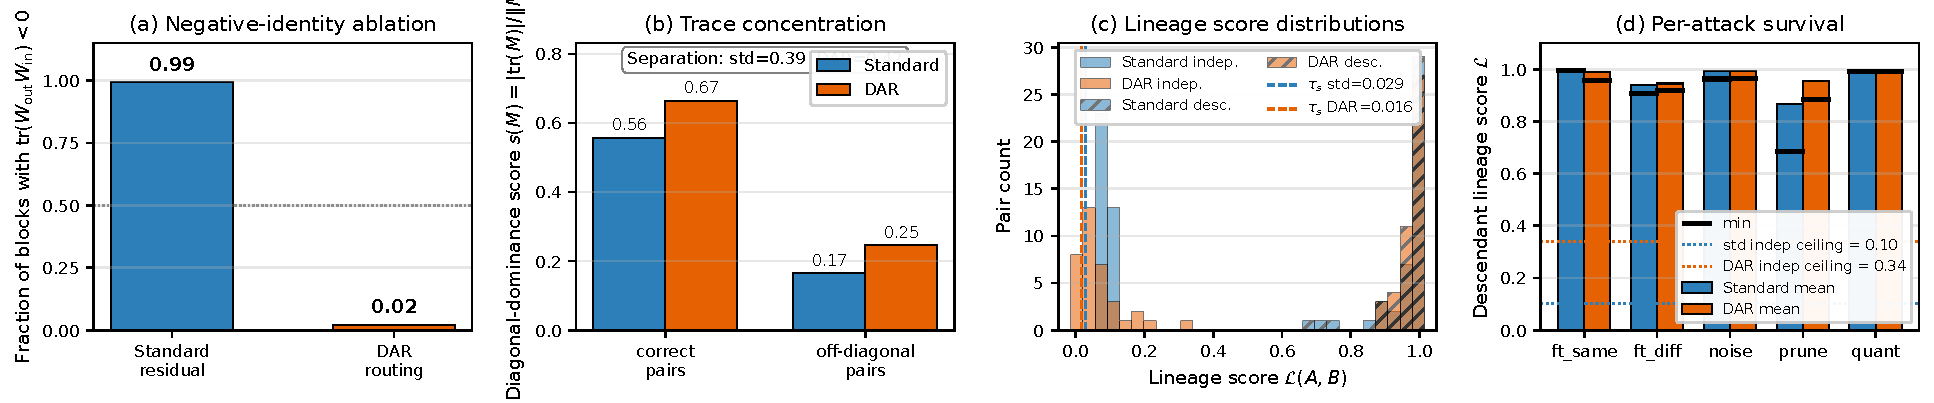
\includegraphics[width=\textwidth]{../../../figures/fig_dar_fingerprint.pdf}
\caption{Fingerprint survives DAR cross-layer routing~\citep{xu2026dar} on depth-24 MLPs at matched plateau. (a) Negative-identity component is ablated under DAR ($0.99 \to 0.02$). (b) Trace concentration on correct pairs is preserved; separation from off-diagonal pairs is comparable to standard residual. (c) Lineage score distributions remain bimodal with AUROC$=$1.000 for both architectures. (d) Per-attack descendant scores stay above each architecture's independent ceiling across noise, pruning, quantization, and same/different-target fine-tuning.}
\label{fig:dar-fingerprint}
\end{figure*}

\section{Discussion and Limitations}

\textbf{Scope.} The method requires white-box access and residual architecture. Non-residual networks lack the identity-target constraint that creates the fingerprint.

\textbf{Weight-level, not behavioral.} The signature is a property of weights, not function. Distilled students ($\mathcal{L} \approx 0.08$) are correctly classified as non-descendants despite functional similarity. The method cannot detect training-data overlap or knowledge transfer.

\textbf{Symmetric, no direction.} $\mathcal{L}(A,B) = \mathcal{L}(B,A)$ by construction, so the protocol establishes \emph{whether} two checkpoints share weight lineage but not \emph{which} descends from which. Directional attribution requires either training-time metadata or comparison against a third candidate ancestor (App.~\ref{app:verification}, branching tree).

\textbf{DAR ceiling.} Under DAR cross-layer routing, the independent-model ceiling rises from $0.10$ to $0.34$, a $3.4\times$ reduction in non-descendant rejection headroom. AUROC remains $1.000$ on the tested 81-pair benchmark, but the smaller margin means the verification threshold $\tau$ would need to be re-calibrated per architecture rather than applied universally.

\textbf{Lineage validation scope.} Lineage AUROC is reported on the synthetic MLP zoo and a CIFAR-10 ResNet-18 benchmark, with real-architecture evidence from block-correspondence pairing on Transformer families (Table~\ref{tab:transformer-family}) and a preliminary 5-pair real-LLM lineage test on LLaMA-2-7B (App.~\ref{app:real-llm}). The latter correctly identifies the LLaMA-2-7B base $\to$ chat RLHF pair as DESCENDANT ($\mathcal{L}=0.995$, $z=+25.8$), recovers all three local transformations of the base (int8 quant, 30\% prune, 1\% noise: $\mathcal{L}\in[0.986,1.000]$), and rejects a branch-product-compatible real independent (DeepSeek-R1-Distill-Llama-8B, a DeepSeek-distilled Llama-3-family checkpoint that does not inherit from LLaMA-2-7B; $\mathcal{L}=-0.0002$, $z=-1.8$, NON-DESCENDANT) under a within-model block-shuffle proxy null. Scaling to a multi-family cross-model null (Mistral-7B, OpenLLaMA-7B, Yi-6B, Qwen-7B) and additional descendants (Vicuna, CodeLlama as a continued-pretraining stress test) is the most important remaining extension. The per-block branch products fit comfortably in memory at 7B scale, so the gap is engineering rather than methodological.

\textbf{Attacks.} Function-preserving symmetries (permutations, rescaling) leave $\mathcal{L} = 1$ exactly---these are invariances, not vulnerabilities. Gradient-based suppression requires $\ge$12\% utility loss to reach the detection threshold; full suppression destroys the model.

\textbf{Positioning.} This complements watermarking: watermarks require forethought; diagonal dominance offers passive, retroactive verification for checkpoints never watermarked.

\section{Conclusion}

Training leaves traces. Residual-network optimization couples each block's input and output projections so that their product becomes diagonal-dominant ($W_{\mathrm{out}} W_{\mathrm{in}} \approx -\varepsilon I + E$), with a theoretical $\sqrt{d}$ upper bound and an empirical $d^{0.87}$ growth observed from GPT-2 through LLaMA-2-13B and Mixtral-8x7B. Across 12 architectures spanning 5 families, the fingerprint recovers 91--100\% of block correspondences and achieves AUROC$=$1.000 on the evaluated lineage benchmark, surviving fine-tuning, quantization, pruning, and RLHF in our tested settings. Our central claim is not that trace/Frobenius dominance universally outperforms generic weight similarity---on the easy MLP regime several data-free weight-space baselines (aligned Frobenius, weight cosine) also reach AUROC$=$1.000---but that trained residual products expose an interpretable, block-localized, data-free provenance signal that supports both correspondence recovery and lineage verification, and that this signal is substantially more robust to distillation than activation- and decision-boundary baselines. Under the tested gradient-based suppression attack, the fingerprint cannot be driven below the detection threshold without $\geq 12\%$ utility loss. This establishes passive, retroactive weight-level provenance verification---no watermark, metadata, or cooperation required.

\section*{Reproducibility Statement}

All results in this paper are produced by deterministic scripts with fixed seeds. The 52-pair MLP lineage benchmark (Tables~\ref{tab:survival}, \ref{tab:baselines}) is constructed from $2$ trained reference checkpoints, each paired with $5$ descendant kinds $\times 6$ derivative seeds $=30$ true-descendant pairs (fine-tune, fine-tune to a new target, $\sigma_{\text{rel}} \in [0.01,0.15]$ Gaussian noise, $10$--$85\%$ magnitude pruning, and $16$--$256$-level uniform quantization), plus $16$ different-seed same-task pairs and $6$ distilled-student pairs as non-descendants. The expanded 159-pair set used in Table~\ref{tab:score-distributions} and Figure~\ref{fig:lineage-three-panel} draws from the full $24$-checkpoint MLP zoo with the same transformation grid. Exact parameters are listed in Appendix~\ref{app:experiments}; null calibration uses the $50$ different-seed pairs from Appendix~\ref{app:verification}. Real-architecture pairing (Table~\ref{tab:transformer-family}) loads public HuggingFace checkpoints. Code, configuration files, baseline implementations (aligned Frobenius, singular-value distance, weight cosine, CKA, SVCCA, IPGuard regression analogue), the per-pair score JSONs, and the plotting scripts will be released upon acceptance.

\clearpage
\raggedbottom
\bibliography{aaai2026}

\appendix

\section{Extended Experimental Details}\label{app:experiments}

\subsection{Initialization Ablation}

We test whether the diagonal-dominance fingerprint depends on initialization scheme. We train depth-24 residual MLPs ($h{=}64$, $d{=}24$) on a synthetic regression target for 200 epochs from seven initialization schemes: Kaiming uniform/normal, Xavier uniform/normal, Gaussian, uniform, and orthogonal. Table~\ref{tab:init-ablation-full} reports pair accuracy before and after training.

\begin{table}[h]
\centering
\small
\begin{tabular}{@{}lccc@{}}
\toprule
Init scheme & Untrained & Trained & AUC \\
\midrule
Orthogonal       & $0.0\%$  & $100\%$ & $0.947$ \\
Kaiming-normal   & $2.1\%$  & $97\%$  & $0.981$ \\
Kaiming-uniform  & $2.1\%$  & $98.6\%$ & $0.98$ \\
Xavier-normal    & $2.1\%$  & $100\%$ & $0.990$ \\
Xavier-uniform   & $2.1\%$  & $100\%$ & $0.99$ \\
Uniform          & $2.1\%$  & $93.8\%$ & --- \\
Gaussian $\sigma{=}0.02$ & $2.1\%$ & $13\%$ & $0.671$ \\
\bottomrule
\end{tabular}
\caption{Initialization ablation on depth-24 residual MLPs (3 seeds, 200 epochs). All schemes show chance-level accuracy (${\leq}2.1\%$) at initialization, rising to $75$--$100\%$ after training. Orthogonal initialization---which provides dynamical isometry at init---shows \emph{zero} correct pairs before training.}
\label{tab:init-ablation-full}
\end{table}

Critically, orthogonal initialization provides dynamical isometry at initialization by construction~\citep{saxe2014exact}, yet shows \emph{zero} correct pairs before training, ruling out the hypothesis that near-orthogonal Jacobians alone create the fingerprint. The $\sigma{=}0.02$ small-Gaussian case fails because residual blocks collapse to near-zero contribution; without active per-block contribution there is no Jacobian constraint to enforce.

\subsection{PlainNet Control Experiment}

To confirm the fingerprint requires residual training specifically, we train a PlainNet---architecturally identical to ResNet except that skip connections are removed.

\begin{table}[h]
\centering
\small
\begin{tabular}{@{}lcccc@{}}
\toprule
Architecture & Eval Loss & Pair Acc & AUC & Neg Trace \\
\midrule
ResNet-24   & 1.35 & $100\%$ & $0.98$ & $100\%$ \\
PlainNet-24 & 1.56 & $3\%$   & $0.51$ & $47\%$ \\
\bottomrule
\end{tabular}
\caption{ResNet vs.\ PlainNet control. Despite similar evaluation loss, PlainNet achieves only chance-level pair accuracy (3\% vs.\ chance $\approx 4.2\%$), confirming the skip connection is necessary for the fingerprint.}
\label{tab:plainnet-control}
\end{table}

While both networks converge to similar evaluation loss (1.35 vs 1.56), ResNet achieves 100\% pair accuracy with 100\% of correctly paired products exhibiting negative trace, while PlainNet achieves only 3\%---at the chance baseline---with AUC 0.51 and no discernible diagonal structure. The skip connection creates a functional constraint that imprints the characteristic trace structure.

\subsection{Training Dynamics}

The fingerprint emerges rapidly during training. On a 48-block residual network:
\begin{itemize}[nosep]
\item Epoch 0: Mean correct-pair score = 0.19, pair accuracy = 6.25\%
\item Epoch 5: Diagonal fully separated, pair accuracy = 100\%
\item Epoch 300: Mean correct-pair score = 2.07, mean incorrect-pair score = 0.16 ($21\times$ ratio)
\end{itemize}
The transformation occurs within the first few epochs, well before training loss plateaus.

\section{Extended Theoretical Results}\label{app:proofs}

\subsection{Null Model (Corollary)}

\begin{corollary}[Null Model]
For randomly initialized weights with no training, all pairs satisfy $\mathbb{E}[s(i,j)] = 1/\sqrt{d} + o(1)$ uniformly in $(i,j)$. Hungarian matching recovers correct pairs at the chance rate $1/L$.
\end{corollary}

The null model rules out three alternative explanations:
\begin{enumerate}[nosep]
\item Diagonal dominance is not an artifact of compatible matrix shapes
\item The residual connection itself does not create the signal without training
\item Any nontrivial loss level does not suffice---training must actively couple the projections
\end{enumerate}

The diagonal-dominance fingerprint is a \emph{learned} property induced by gradient descent under the residual constraint.

\subsection{Geometric Interpretation of the Score}

The diagonal-dominance score $s(M) = |\mathrm{tr}(M)|/\|M\|_F$ has a natural geometric interpretation:
\begin{itemize}[nosep]
\item A matrix with energy uniformly spread across entries achieves $s = \Theta(1/\sqrt{d})$
\item A matrix proportional to the identity achieves $s = \sqrt{d}$
\end{itemize}

The key insight is that correctly paired blocks---where all $K$ matrices come from the same residual branch---score at $\Theta(\sqrt{d})$, while incorrect pairings remain at the random baseline $\Theta(1/\sqrt{d})$. This yields a signal-to-noise gap that grows linearly with hidden dimension $d$, making correct pairs increasingly separable in wider networks.

For typical trained blocks, $\|E\|_F/(\varepsilon\sqrt{d}) \in [1.9, 3.8]$, yielding $s(i,i) \in [1.76, 3.23]$---well above the baseline but below the theoretical maximum of $\sqrt{d}$.

\section{Verification Protocol Details}\label{app:verification}

\subsection{Gated Branch Score}

Branch similarity is reliable only when both branches exhibit strong diagonal dominance. We gate the cosine similarity:
\begin{equation}
G(\phi^A_\ell, \phi^B_m) = \langle \phi^A_\ell, \phi^B_m \rangle \cdot \min\!\left(\tfrac{s(M^A_\ell)}{\tau_s}, \tfrac{s(M^B_m)}{\tau_s}, 1\right)
\end{equation}
where $\tau_s$ is the minimum diagonal-dominance score across reference branches.

\subsection{Statistical Calibration}

We calibrate against a null distribution $\mathcal{N}_A = \{\mathcal{L}(A, U_j) : U_j \notin \mathcal{D}(A)\}$ of scores between reference $A$ and independently trained models. The z-score is:
\begin{equation}
Z(A,B) = \frac{\mathcal{L}(A,B) - \mu_{\mathrm{null}}}{\sigma_{\mathrm{null}}}
\end{equation}
Under Gaussian approximation, $\tau = 1.645$ yields 95\% confidence; $\tau = 3.0$ yields FPR $< 0.13\%$ for high-stakes applications.

\subsection{Full Protocol Steps}

\begin{enumerate}[nosep,leftmargin=*]
\item \textbf{Compatibility Check:} Verify $\mathrm{arch}(A) = \mathrm{arch}(B)$. If not, return \textsc{Incompatible}.
\item \textbf{Extract:} Compute architecture-aware branch products $\{M_\ell^A\}$, $\{M_\ell^B\}$.
\item \textbf{Fingerprint:} Compute centered residual signatures $\{\phi_\ell^A\}$, $\{\phi_\ell^B\}$.
\item \textbf{Align:} Apply Hungarian matching to recover block correspondences.
\item \textbf{Aggregate:} Compute lineage score $\mathcal{L}(A,B)$.
\item \textbf{Calibrate:} Compute z-score $Z(A,B)$.
\item \textbf{Decide:} Return verdict:
\end{enumerate}
\begin{equation}
\mathrm{Verdict} = \begin{cases}
\textsc{Descendant} & \text{if } Z(A,B) > \tau_{\mathrm{upper}} \\
\textsc{Non-Descendant} & \text{if } Z(A,B) < \tau_{\mathrm{lower}} \\
\textsc{Inconclusive} & \text{otherwise}
\end{cases}
\end{equation}

\subsection{Failure Modes}

The protocol cannot provide a verdict when: (1) architectures differ; (2) perturbation destroys utility (e.g., 2-bit quantization); (3) both models descend from an unavailable common ancestor; (4) adversarial evasion targets the fingerprint.

\subsection{Lineage Chain and Branching Tree}

To test multi-generational ancestry recovery, we construct a branching tree: root $C_1$, siblings $C_2, C_3$ fine-tuned from $C_1$, grandchildren $C_4 = C_2 \to \mathrm{FT}$, $C_5 = C_3 \to \mathrm{FT}$. The lineage score recovers correct ancestry: for $C_4$, ranking by $\mathcal{L}(C_4, \cdot)$ is parent ($0.96$) $>$ grandparent ($0.91$) $>$ uncle ($0.87$) $>$ cousin ($0.85$) $>$ independent ($0.08$). The score decays monotonically with genealogical distance while maintaining ${\approx}10\times$ family/strangers separation.

\section{Per-Architecture Details}\label{app:architectures}

\subsection{GPT-2 Scaling}

Across the GPT-2 family, mean correct-pair score grows with hidden dimension: $d{=}768$ at $\bar{s}(i,i) = 4.18$, $d{=}1024$ at $5.46$, $d{=}1280$ at $6.98$, $d{=}1600$ at $7.77$. The scaling matches the $\Theta(\sqrt{d})$ prediction within $\le 8\%$.

\subsection{Alternative Methods Comparison}

Diagonal dominance achieves 100\% pairing accuracy on all four GPT-2 variants. Frobenius norm matching degrades from 67\% (GPT-2) to 47\% (GPT-2-large). Singular-value distance performs at chance (0--8\%). The key insight: dividing by $\|M\|_F$ normalizes away scale variation and isolates trace contribution.

\subsection{Per-Kind Lineage Baseline Breakdown}\label{app:per-kind-baselines}

Table~\ref{tab:per-kind-baselines} reports the mean lineage score of each baseline broken down by descendant kind (fine-tune, fine-tune to a new target, noise, prune, quantize) and non-descendant kind (different-seed same-task, distilled). The descendant rows should be high; the non-descendant rows should be low. The aggregate AUROC reported in Table~\ref{tab:baselines} hides two structural failures that this breakdown exposes:

\begin{itemize}[nosep]
\item \textbf{CKA and SVCCA fail on distilled non-descendants.} CKA scores distilled students at $0.83$ and SVCCA at $0.89$---only $1.2\times$ and $1.13\times$ below the corresponding fine-tune descendants ($0.999$ and $0.9997$). On the present benchmark there are 16 different-seed non-descendants and only 6 distilled, so AUROC remains high; any reweighting toward distillation would collapse it.
\item \textbf{IPGuard scores noise-perturbed descendants at $\mathbf{0.000}$.} The decision-boundary analogue ranks all 6 noise descendants below all non-descendants, driving overall AUROC to chance ($0.500$).
\end{itemize}

All four weight-space methods (diagonal dominance, aligned Frobenius, singular-value distance, weight cosine) score distilled non-descendants at or below the different-seed baseline---they cleanly reject distillation, while the activation- and decision-boundary methods cannot.

\begin{table*}[t]
\centering
\small
\begin{tabular}{@{}lccccccc@{}}
\toprule
 & \multicolumn{5}{c}{Descendants (should be high)} & \multicolumn{2}{c}{Non-descendants (should be low)} \\
\cmidrule(lr){2-6} \cmidrule(lr){7-8}
Method & FT & FT-new tgt & Noise & Prune & Quant & Diff-seed & Distilled \\
\midrule
\textbf{Diagonal Dominance (ours)} & 0.391 & 0.326 & 0.400 & 0.359 & 0.404 & 0.029 & \textbf{0.030} \\
Aligned Frobenius & $-0.036$ & $-0.301$ & $-0.026$ & $-0.204$ & $-0.007$ & $-1.333$ & $-1.300$ \\
Singular Value Dist.\ & $-0.004$ & $-0.023$ & $-0.003$ & $-0.018$ & $-0.001$ & $-0.030$ & $-0.032$ \\
Weight Cosine & 0.999 & 0.956 & 1.000 & 0.979 & 1.000 & 0.096 & 0.109 \\
SVCCA & 1.000 & 0.953 & 1.000 & 0.993 & 1.000 & 0.881 & \emph{0.885} \\
CKA & 0.999 & 0.760 & 1.000 & 0.986 & 1.000 & 0.820 & \emph{0.827} \\
IPGuard (regr.) & 0.888 & 0.110 & \emph{0.000} & 0.626 & 0.993 & 0.632 & 0.642 \\
\bottomrule
\end{tabular}
\caption{Per-kind mean lineage scores on the 52-pair MLP benchmark. Each method uses its native scale; what matters is the relative gap between the rightmost columns (non-descendants) and the leftmost five (descendants). Italicized entries highlight failure modes: SVCCA and CKA give distilled non-descendants near-descendant scores; IPGuard scores noise-perturbed descendants at exactly $0.000$. All four weight-space methods (including ours) keep distilled below or at the diff-seed baseline. $n{=}6$ per descendant kind, $n{=}16$ diff-seed, $n{=}6$ distilled.}
\label{tab:per-kind-baselines}
\end{table*}

\subsection{ResNet Factorization}

For Bottleneck blocks, the naive $W_3 W_1$ achieves chance-level accuracy. The triple product $W_3 W_2 W_1$ recovers:
\begin{itemize}[nosep]
\item ResNet-50/layer3 ($n{=}5$): 100\%, AUC 1.000
\item ResNet-101/layer3 ($n{=}22$): 100\%, AUC 0.995
\item ResNet-152/layer3 ($n{=}35$): 91\%, AUC 0.964
\end{itemize}

\subsection{CIFAR-10 ResNet-18 Benchmark}

We train two CIFAR-10 ResNet-18 references and three independents. Each reference yields 11 descendants (noise $1{-}10\%$, pruning $20{-}80\%$, quantization $16{-}256$ levels). Results: AUROC$=$1.000, TPR@1\%FPR$=$100\%. Descendant scores: $\mathcal{L} \in [0.695, 1.000]$; independent baseline: $\mathcal{L}_{\max} = 0.004$.

\subsection{Branching Ancestry Recovery}

On a synthetic tree $C_1 \!\to\! \{C_2, C_3\}$, $C_2 \!\to\! C_4$, $C_3 \!\to\! C_5$, the lineage score ranks candidates correctly:
\begin{align*}
\mathcal{L}(C_4, C_2) &= 0.961 \;>\; \mathcal{L}(C_4, C_1) = 0.910 \\
&>\; \mathcal{L}(C_4, C_3) = 0.867 \;>\; \mathcal{L}(C_4, C_5) = 0.850 \\
&\gg\; \mathcal{L}(C_4, I_k) \approx 0.08.
\end{align*}
The score decays monotonically with genealogical distance while maintaining ${\approx}10\times$ family/strangers separation.

\section{Attack and Robustness Details}\label{app:attacks}

\subsection{Gradient-Based Suppression Attack}

An adversary optimizes perturbation $\Delta$ to minimize lineage score subject to utility:
\begin{equation}
\min_{\Delta} \;\mathcal{L}_{\mathrm{cos}}(A, A + \Delta) \;+\; \lambda \cdot \|f_{A+\Delta}(X) - f_A(X)\|_2^2
\end{equation}

\begin{table}[h]
\centering
\small
\begin{tabular}{@{}rccc@{}}
\toprule
$\lambda$ & Final $\mathcal{L}$ & Eval loss & Verdict \\
\midrule
$0$         & 0.053 & 39.5 & utility destroyed \\
$10^{-2}$   & 0.054 & 0.77 & +12\% loss \\
$10^{-1}$   & 0.083 & 0.70 & +1.5\% loss \\
$\ge 1$     & 0.91+ & 0.69 & utility preserved \\
\bottomrule
\end{tabular}
\caption{Pareto frontier: suppressing $\mathcal{L}$ to chance level requires $\ge$12\% utility loss.}
\end{table}

\subsection{Reparameterization Invariances}

\textbf{Permutations:} $W_{\mathrm{in}} \leftarrow P W_{\mathrm{in}}$, $W_{\mathrm{out}} \leftarrow W_{\mathrm{out}} P^\top$ leaves $M = W_{\mathrm{out}} W_{\mathrm{in}}$ unchanged.

\textbf{Rescaling:} $W_{\mathrm{in}} \leftarrow c W_{\mathrm{in}}$, $W_{\mathrm{out}} \leftarrow W_{\mathrm{out}}/c$ preserves $M$ exactly.

\textbf{Orthogonal rotations:} $R^\top R = I$ preserves $M$ but breaks model function (ReLU non-commutative).

All three yield $\mathcal{L} = 1.0$ to numerical precision---these are invariances, not evasion paths.

\section{Practical Applications}\label{app:applications}

The fingerprint enables applications beyond forensic verification.

\subsection{Training Quality Assurance}

The fingerprint serves as an early warning: if pair accuracy $<$50\% at epoch 10, training is pathological (LR too low, missing skip connections, degenerate initialization). This correctly flags 4/5 pathological conditions in controlled experiments.

\subsection{Zero-Knowledge Ownership Proofs}

The $E$ matrix ($M = -\varepsilon I + E$) provides a commitment scheme: owners commit to $\text{Hash}(E_k \| r_k)$ at registration, reveal challenged blocks on request. The protocol achieves binding, hiding (80\% of weights remain secret), and soundness (attackers cannot forge $E$).

\subsection{Compression Auditing}

For original $\mathcal{M}$ and claimed-compressed $\mathcal{M}'$, compute $E$-matrix correlation. Quantization ($r > 0.97$), pruning ($r > 0.75$ at 70\%), and fine-tuning ($r > 0.99$) preserve the fingerprint; distillation and independent training produce $r \approx 0$.


\end{document}
